\documentclass[journal]{IEEEtran}

%%%%%%%%%%%%%%%%%%%%%%%%%%%%%%%%%%%%%%%%%%%%%%%%%%
%%%%% Packages %%%%%%%%%%%%%%%%%%%%%%%%%%%%%%%%%%%
%%%%%%%%%%%%%%%%%%%%%%%%%%%%%%%%%%%%%%%%%%%%%%%%%%

\usepackage[utf8]{inputenc}
\usepackage[T5]{fontenc}   

\usepackage[style=ieee, backend=biber, natbib=true]{biblatex}
\bibliography{references.bib} 
\usepackage[colorlinks=true, allcolors=blue]{hyperref}

\usepackage{amsmath}
\usepackage{url}
\hyphenation{op-tical net-works semi-conduc-tor}
\usepackage{graphicx}
\usepackage{float}
\usepackage{dblfloatfix}% http://ctan.org/pkg/dblfloatfix
\usepackage{multicol}% http://ctan.org/pkg/multicols
\usepackage{tabularx}

%%%%%%%%%%%%%%%%%%%%%%%%%%%%%%%%%%%%%%%%%%%%%%%%%%

\renewcommand{\ttdefault}{lmtt}              

\makeatletter

\renewcommand{\abstract}{\textbf{Tóm tắt:}}
\renewcommand{\IEEEkeywords}{\textbf{Từ khoá:}}
\renewcommand{\appendices}{\section*{Phụ lục}}
\renewcommand{\figurename}{Hình}
\renewcommand{\tablename}{BẢNG} 

\begin{document}
	
	\title{Định danh chủng vi khuẩn tiềm năng chứa gen oxy hoá arsenite \textit{aioA} trong môi trường đất tại Việt Nam}
	
	\author{Hoàng Xuân Tùng \\
		{\small Lớp Tin Sinh học 752510, Trường Hoá và Khoa học Sự sống, Đại học Bách khoa Hà Nội}
	}
	
	\markboth{Tin sinh học}%do not delete next lines
	{Shell \MakeLowercase{\textit{et al.}}: Bare Demo of IEEEtran.cls for IEEE Journals}
	
	\maketitle
	
	\begin{abstract}
		\textbf{Việc xác định các chủng vi sinh vật có khả năng oxy hóa arsenite đóng vai trò quan trọng trong nghiên cứu xử lý ô nhiễm kim loại nặng tại Việt Nam. Trong nghiên cứu này, một chủng vi khuẩn tiềm năng đã được phân lập từ môi trường đất và định danh dựa trên trình tự gen 16S rRNA. Phân tích {\footnotesize BLASTN} và phát sinh loài cho thấy chủng này có quan hệ gần gũi với \textit{Ancylobacter novellus} và thuộc chi \textit{Ancylobacter}. Để kiểm tra sự hiện diện của gen \textit{aioA}, một gen chức năng liên quan đến khả năng oxy hoá arsenite, các trình tự ortholog từ các loài gần gũi đã được thu thập và phân tích nhằm xác định vùng bảo tồn. Một cặp mồi đặc hiệu đã được thiết kế và đánh giá về tính đặc hiệu cũng như các đặc tính lý hoá. Ngoài ra, protein được mã hoá bởi gen \textit{aioA} cũng được phân tích đặc điểm sinh hoá và dự đoán cấu trúc không gian ba chiều. Những kết quả thu được nhằm tạo nền tảng cho việc sàng lọc hiệu quả các chủng vi sinh vật tiềm năng và mở ra triển vọng ứng dụng chúng trong các chiến lược xử lý arsenite ngoài thực địa một cách chính xác và bền vững.}
	\end{abstract}
	
	\begin{IEEEkeywords}
		16S rRNA, \textit{aioA}, phát sinh loài, thiết kế mồi.
	\end{IEEEkeywords}
	
	\section{Mở đầu}
	
	Các loài \textit{Ancylobacter} sp. trước đây được phân loại trong chi \textit{Microcyclus} của họ \textit{Spirosomaceae} \cite{orskov1928beschreibung}, chúng là những vi khuẩn hình que cong, hiếu khí bắt buộc, Gram âm. Tuy nhiên, những tiến bộ gần đây trong công nghệ định danh sinh vật và phân tích phát sinh loài đã mang lại những hiểu biết mới về đặc điểm di truyền và phân loại của chi này. Phân tích phát sinh loài dựa trên trình tự 16S rRNA đã chỉ ra rằng các các loài thuộc chi \textit{Ancylobacter} là thành viên của lớp \textit{Alphaproteobacteria} \cite{woese1990phylogenetic}. Các thành viên thuộc chi \textit{Ancylobacter} thường được tìm thấy trong môi trường đất và nước ngọt. Trên môi trường rắn, khuẩn lạc của chúng có màu trắng kem; ở môi trường lỏng, chúng hình thành màng nổi. Các chủng đều dương tính với phản ứng oxidase và catalase \cite{larkin1977taxonomy}. \textit{Ancylobacter} là nhóm vi khuẩn dị dưỡng hóa học, methylotrophic tùy nghi, có khả năng sử dụng đa dạng các loại đường và muối của acid hữu cơ làm nguồn carbon, một số chủng còn thể hiện khả năng hóa dưỡng vô cơ khi sử dụng hydro phân tử \cite{namsaraev1978autotrophic}. Hiện tại, chi \textit{Ancylobacter} bao gồm hơn 22 loài được công bố hợp lệ (\href{(https://lpsn.dsmz.de/genus/ancylobacter}{https://lpsn.dsmz.de/genus/ancylobacter}). Nghiên cứu gần đây đã nhấn mạnh ứng dụng tiềm năng của các loài \textit{Ancylobacter} như khả năng khử halogen \cite{firsova2009ancylobacter}, phân hủy các hợp chất hữu cơ như 1,2-dichloroethane  \cite{wu2025characterization} và 2-chloroethylvinylether \cite{van1993degradation}, sản xuất cellulose năng suất cao \cite{martirani2025spontaneous} và oxi hoá arsenite \cite{andreoni2012arsenite,battaglia2002arsenic}.
	
	Ở điều kiện tự nhiên, arsenite (AsIII) là một trong hai dạng tồn tại chính của arsenic trong môi trường. Loại As(III) trên đã được chứng minh là gây độc hại đến các quá trình trao đổi chất của sinh vật sống như ức chế hệ thống enzyme, ức chế sự sửa chữa DNA và hô hấp ty thể, gây ra nhiều phản ứng căng thẳng, thúc đẩy khuếch đại gen và tạo tổn thương di truyền \cite{snow1999modulation}. Trong khi đó, đối với nhiều chủng vi khuẩn oxy hóa arsenite dị dưỡng và hoá dưỡng, quá trình oxy hóa As(III) thông qua hệ thống enzyme Aio (gồm hai tiểu đơn vị AioA và AioB với gen mã hoá các tiểu đơn vị tương ứng là \textit{aioA}, \textit{aioB}) \cite{mukhopadhyay2002microbial, yamamura2014microbiology} lại được coi là một cơ chế giải độc, một nguồn năng lượng bổ sung để phát triển khi có carbon dioxide trong điều kiện hiếu khí \cite{bryan2009carbon,duquesne2008arsenite,garcia2008novel,santini2000new} và khử nitrat \cite{oremland2002anaerobic}. Đồng thời với việc gen \textit{aioA} đã được sử dụng để làm chất đánh dấu phân tử để khảo sát sự đa dạng và phân loại các cộng đồng vi sinh vật oxy hóa As(III) trong môi trường \cite{zhang2017nitrate, xue2020microbial, zhai2020abundance}, vi sinh vật đã được tạo điều kiện mạnh mẽ để trở thành những ứng cử viên tiềm năng cho việc phân huỷ arsenite trong các khu vực ô nhiễm với hiệu quả cao, quy mô lớn với chi phí tiết kiệm. Cho đến nay, các gen tương đồng mã hóa AioAB đã được tìm thấy đa dạng ở các chủng thuộc Actinobacteria, Aquificae, Bacteroidetes, Chlorobi, Chloroflexi, Crenarchaeota, Deinococcus-Thermus, Firmicutes, Nitrospira và  $\alpha$-, $\beta$-, $\gamma$-Proteobacteria \cite{yamamura2014microbiology}. Mục tiêu của bài báo cáo này là định danh chủng vi khuẩn được cho là thuộc chi \textit{Ancylobacter} dựa trên gen mã hoá 16S rRNA và thiết kế mồi cho phản ứng PCR để xác định sự có mặt của gen \textit{aioA} trong chủng vi sinh vật này.
	
	\section{Nguyên liệu và phương pháp}
	
	\subsection{Định danh chủng vi sinh vật}
	
	Chủng vi sinh vật đã được phân lập từ môi trường tự nhiên với trình tự gen được xác định thông qua phương pháp giải trình tự Sanger hai chiều. Trình tự consensus của đoạn gen mã hoá 16S rRNA được thiết kế thông qua phần mềm {\footnotesize MEGA12} phiên bản 12.0.11 \cite{kumar2024mega12} và được khuếch đại bằng cặp mồi 27F/1492R \cite{frank2008critical}. Phân tích {\footnotesize BLASTN} với cơ sở dữ liệu trình tự rRNA/ITS/16S rRNA của vi khuẩn và cổ khuẩn đã loại trừ các trình tự thu thập từ môi trường \cite{altschul1990basic} được sử dụng để xác định các loài có quan hệ gần gũi.
	
	\subsection{Xây dựng cây phát sinh loài dựa trên gen 16S rRNA}
	
	Vị trí phân loại của chủng được xác định dựa trên cơ sở dữ liệu Taxonomy của NCBI \cite{schoch2020ncbi}. Để làm sáng tỏ mối quan hệ phát sinh loài giữa chủng C3 và các loài liên quan, một cây phát sinh loài được xây dựng trên trình tự 16S rRNA. Phân tích bao gồm các loài thuộc chi \textit{Ancylobacter}, cũng như các chi liên quan của nó là \textit{Aquabacter}, \textit{Xanthobacter}, \textit{Azorhizobium} và \textit{Labrys}. Bộ dữ liệu gen 16S rRNA đã được căn chỉnh bằng {\footnotesize CLUSTALW} \cite{thompson1994clustal} và các mối quan hệ phát sinh loài đã được suy ra bằng phương pháp neighbor-joining (NJ) \cite{kumar2024mega12}. Cấu trúc tôpô của cây đã được đánh giá bằng phương pháp bootstrap với 1000 lần lấy mẫu lặp lại, với \textit{Escherichia coli} VANM 2 được sử dụng làm nhóm ngoài (outgroup). 
	
	\subsection{Thiết kế mồi khuếch đại gen \textit{aioA}}
	
	Để kiểm tra sự hiện diện của gen chức năng ở chủng vi sinh vật được phân lập, cặp mồi PCR đã được thiết kế dựa trên vùng bảo thủ của các ortholog có chức năng quan tâm được chú thích từ các loài có quan hệ gần gũi. Các trình tự ortholog thuộc họ Xanthobacteraceae (Bảng~\ref{table_2}), bao gồm các loài trong chi \textit{Rhizobium}, \textit{Shinella} và \textit{Sinorhizobium}, đã được thu thập từ cơ sở dữ liệu NCBI GenBank. Trong đó, \textit{Ancylobacter} sp. TS-1 được chọn làm chủng tham chiếu gần gũi nhất về mặt phân loại với chủng nghiên cứu. Các trình tự thu được đã được căn chỉnh bằng cách sử dụng chương trình {\footnotesize CLUSTAL OMEGA} của EBI \cite{sievers2011fast} và phân tích đa trình tự nhằm xác định các vùng bảo tồn trong gen \textit{aioA} giữa các chủng vi khuẩn. Sau khi xác định được các vùng bảo tồn, cặp mồi đã được thiết kế bằng công cụ NCBI Primer-BLAST (\href{https://www.ncbi.nlm.nih.gov/tools/primer-blast/index.cgi}{https://www.ncbi.nlm.nih.gov/tools/primer-blast}) \cite{ye2012primer}.
	
	\renewcommand{\arraystretch}{1.35}
	
	\begin{table}[h]
		\centering
		\caption{Tám trình tự ortholog với \textit{Ancylobacter} được sử dụng để so sánh và từ đó xác định được vùng bảo thủ.} \label{table_2}
		\noindent
		\begin{tabularx}{0.49\textwidth}{Xr}
			\hline
			\textbf{Tên chủng} & \textbf{Số hiệu truy cập} \\ \hline
			
			\textit{Ancylobacter} sp. TS-1          & KX250215.1                                  \\
			
			\textit{Rhizobium} sp. YE2-4            & KT992350.1                                  \\
			
			\textit{Rhizobium} sp. K3               & KT992346.1                                  \\
			
			\textit{Rhizobium} sp. 3AM-13           & KT992341.1                                  \\
			
			\textit{Rhizobium} sp. Cug7             & MF621580.1                                  \\
			
			\textit{Rhizobium} sp. Cug6             & MF621579.1                                  \\
			
			\textit{Shinella} sp. C23               & KT992342.1                                  \\
			
			\textit{Shinella} sp. Cug3              & MF621576.1                                  \\
			
			\textit{Sinorhizobium} KGO-5            & AB915361.1                                   \\ \hline
			
		\end{tabularx}
	\end{table}
	
	Trình tự protein được chuyển đổi từ trình tự gen mã hoá thông qua công cụ Translate của {\footnotesize EXPASY} \cite{gasteiger2003expasy} và được tính toán khối lượng phân tử cũng như điểm đẳng điện thông qua công cụ Compute pI/Mw {\footnotesize EXPASY} \cite{bjellqvist1993focusing,bjellqvist1994reference,gasteiger2005protein}. Xác định sự có mặt của đoạn trình tự tín hiệu cho việc vận chuyển qua màng tế bào của protein sau dịch mã thông qua chương trình {\footnotesize SIGNALP 6.0} \cite{teufel2022signalp}. Khả năng gắn màng của protein được kiểm tra bằng công cụ {\footnotesize DEEPTMHMM 1.0} \cite{hallgren2022deeptmhmm}. Cấu trúc thực nghiệm của protein được xác minh thông qua đối chiếu với cơ sở dự liệu Protein Data Bank \cite{berman2000protein} và được dự đoán bằng mô hình {\footnotesize ALPHAFOLD} \cite{jumper2021highly} dựa vào chuỗi trình tự thu được từ đoạn gen mã hoá.
	
	\section{Kết quả và thảo luận}
	
	\subsection{Phân tích cây phát sinh loài dựa trên gen 16S rRNA}
	
	Kết quả ở Bảng~\ref{table_1} cho thấy trình tự 16S rRNA của chủng C3 thể hiện mức độ tương đồng cao nhất (99.25\%) với \textit{A. novellus}, tiếp theo là \textit{A. koreensis} (99.10\%), \textit{A. lacus} (97.97\%), \textit{A. defluvii} (97.75\%) và \textit{A. plantiphilus} (97.67\%). Dựa vào cơ sở dữ liệu Taxonomy, vị trí phân loại của chủng nghiên cứu được xác định là thuộc bộ \textit{Hyphomicrobiales}, họ \textit{Xanthobacteraceae}, chi \textit{Ancylobacter}. Như thể hiện trong Hình~\ref{fig:tree}, cây phát sinh loài dựa trên trình tự 16S rRNA chỉ ra rằng các chủng thuộc chi \textit{Ancylobacter} tạo thành một nhánh riêng biệt, với chúng thể hiện mối quan hệ họ hàng gần gũi với \textit{Aquabacter} và \textit{Xanthobacter} hơn là với \textit{Escherichia}. Trong nhánh \textit{Ancylobacter}, chủng C3 có quan hệ họ hàng gần với \textit{A. novellus} DSM 506 và \textit{A. koreensis} NBRC 100963.
	
	\renewcommand{\arraystretch}{1.35}
	
	\begin{table}[h]
		\caption{So sánh độ tương đồng trình tự gen 16S rRNA của chủng C3 với các chủng khác thuộc chi \textit{Ancylobacter} sử dụng BLASTN.} \label{table_1}
		\begin{tabularx}{0.49\textwidth}{Xcr}
			\hline
			\textbf{Tên loài/chủng} & \textbf{Tỷ lệ tương đồng (\%)} & \textbf{Số hiệu truy cập} \\ \hline
			
			\textit{A. novellus} DSM 506        & 99.25                                          & NR\_074219.1                                   \\
			
			\textit{A. koreensis}               & 99.10                                          & NR\_113962.1                                   \\
			
			\textit{A. koreensis}               & 99.10                                          & NR\_041013.1                                   \\
			
			\textit{A. novellus} DSM 506        & 98.50                                          & NR\_025859.1                                   \\
			
			\textit{A. lacus}                   & 97.97                                          & NR\_180559.1 \\
			
			\textit{A. defluvii}                & 97.75                                          & NR\_133695.1                                   \\
			
			\textit{A. plantiphilus}            & 97.67                                          & NR\_180560.1                                   \\
			
			\textit{A. rudongensis}             & 97.68                                          & NR\_029047.1                                   \\
			
			\textit{A. dichloromethanicus}      & 97.60                                          & NR\_116379.1                                   \\
			
			\textit{A. oerskovii}               & 97.52                                          & NR\_042655.1                                   \\ \hline
		\end{tabularx}
	\end{table}
	
	Việc xác định chính xác vị trí phân loại của chủng vi sinh vật là cơ sở quan trọng cho việc suy luận các đặc tính sinh học liên quan, đặc biệt trong bối cảnh nhiều loài thuộc chi này đã được ghi nhận có khả năng oxy hóa arsenite trong môi trường. Dữ liệu phát sinh loài cũng hỗ trợ việc lựa chọn các chủng tham chiếu phù hợp để phân tích gen chức năng.
	
	\begin{table*}[h]
		\caption{Thông số đoạn mồi được thiết kế dựa trên chủng tham chiếu \textit{Ancylobacter} sp. TS-1 thông qua Primer-BLAST. Chiều dài sản phẩm: 360.} \label{table_3}
		\begin{tabularx}{1\textwidth}{lllccccccc}
			\hline
			\textbf{}               & \textbf{Sequence (5' - 3')} & \textbf{Template strand} & \textbf{Length} & \textbf{Start} & \textbf{Stop} & \textbf{Tm} & \textbf{GC\%} & \textbf{Self Comp.} & \textbf{Self 3' Comp.} \\ \hline
			\textbf{Forward primer} & GTGCACATCGTCATCAA           & Plus                     & 17              & 103            & 119           & 52.32       & 47.06         & 6.00                          & 0.00                             \\
			\textbf{Reverse primer} & GCCCCAAAATAGAGCTTG          & Minus                    & 18              & 422            & 405           & 53.34       & 50.00         & 4.00                          & 2.00     \\ \hline                       
		\end{tabularx}
	\end{table*}
	
	\href{}{}
	
	\begin{figure*}[t]
		\centering
		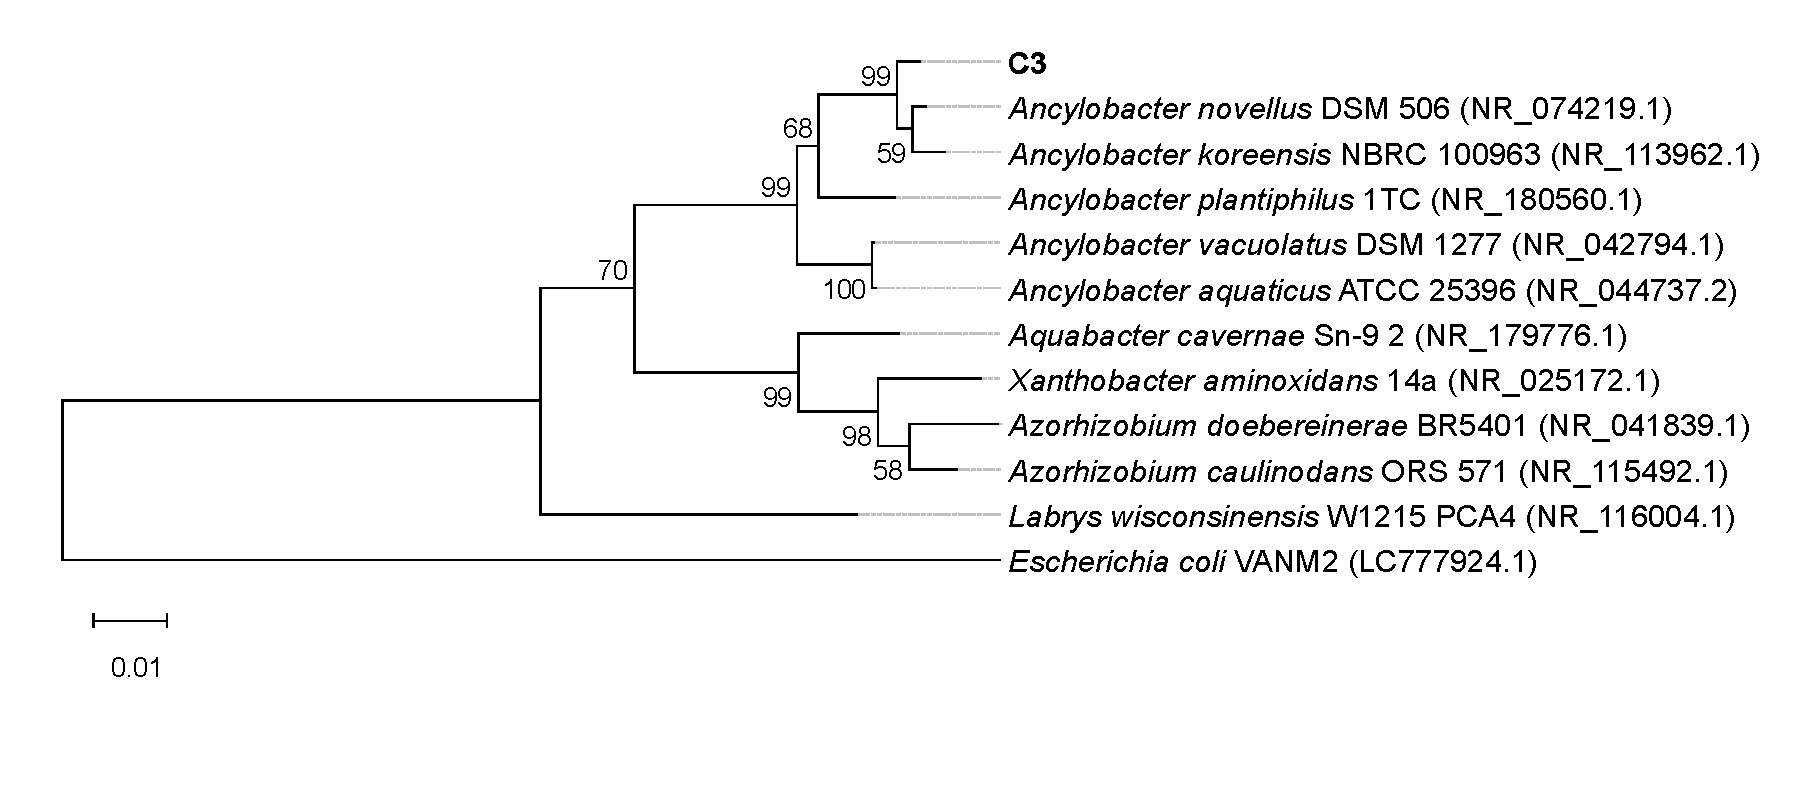
\includegraphics[width=0.95\linewidth]{images/tree.pdf}
		\caption{Cây phát sinh loài theo phương pháp NJ dựa trên trình tự gen 16S rRNA, mô tả mối quan hệ phát sinh loài giữa chủng C3 và các loài gần gũi. Các con số tại các nút nhánh biểu thị giá trị bootstrap 1000 lần lặp lại, chỉ hiển thị các giá trị > 50. Thang tỷ lệ biểu thị 0.01 biến đổi trên mỗi vị trí nucleotide.}
		\label{fig:tree}
	\end{figure*}
	
	\subsection{Đánh giá đoạn mồi khuếch đại gen \textit{aioA}}
	
	Phân tích đa trình tự cho thấy hai vùng bảo tồn nổi bật nằm tại vị trí nucleotide 103–122 và 403–422 trên trình tự gen \textit{aioA} của \textit{Ancylobacter} sp. TS-1, tương ứng với các đoạn trình tự GTGCACATCGTCATCAAGCC và GGCAAGCTCTATTTTGGGGC. Dựa trên hai vùng này, một cặp mồi đã được thiết kế gồm mồi xuôi GTGCACATCGTCATCAA và mồi ngược GCCCCAAAATAGAGCTTG (Bảng~\ref{table_3}). Cặp mồi này đã được kiểm tra lại bằng công cụ {\footnotesize BLASTN} để đảm bảo tính đặc hiệu cao đối với gen \textit{aioA}, với các thông số như nhiệt độ nóng chảy phù hợp, hàm lượng GC nằm trong khoảng tối ưu và không hình thành cấu trúc thứ cấp.
	
	Chiến lược thiết kế mồi dựa trên ortholog giúp mở rộng khả năng áp dụng cặp mồi với các chủng vi khuẩn khác trong họ \textit{Xanthobacteraceae}, đặc biệt có lợi trong các khảo sát đa dạng vi sinh vật môi trường, nơi trình tự gen đích có thể biến đổi nhẹ giữa các loài. Tuy nhiên, nghiên cứu vẫn cần thực nghiệm PCR và giải trình tự để xác minh sự hiện diện và hoạt động của gen trong chủng C3.
	
	\subsection{Phân tích đặc điểm protein được mã hoá bởi gen \textit{aioA}}
	
	\begin{figure}[h]
		\centering
		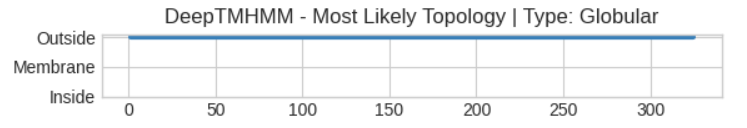
\includegraphics[width=1\linewidth]{images/pro1.png}
		\caption{Khảo sát khả năng gắn trên màng tế bào của protein bằng DeepTMHMM-1.0.}
		\label{fig:pro1}
	\end{figure}
	
	\begin{figure}[h]
		\centering
		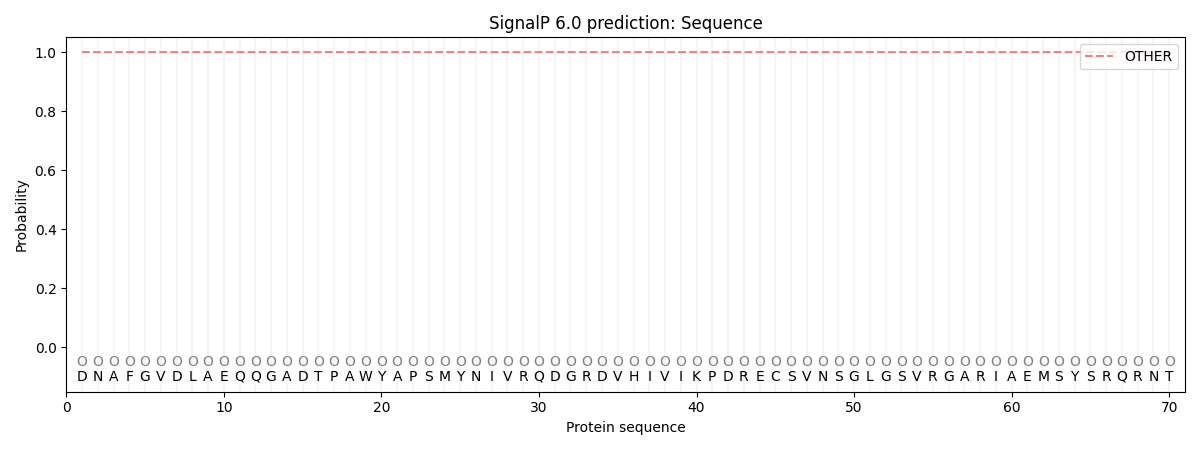
\includegraphics[width=1\linewidth]{images/pro2.png}
		\caption{Khảo sát tín hiệu cho việc vận chuyển qua màng tế bào của protein bằng công cụ SignalP 6.0. Quá trình cải biến sau dịch mã xảy ra ở một số loại protein và chuyển hóa tiền-protein thành dạng có hoạt tính hoặc vận chuyển protein đến vị trí mà tại đó nó có hoạt tính xúc tác (ví dụ như trên màng tế bào, hoặc trong periplasmic). Một trong các quá trình cải biến protein sau dịch mã là vận chuyển protein qua màng tế bào, thông thường, các protein này có một đoạn trình tự peptide làm tín hiệu, sau khi protein được vận chuyển qua màng ra môi trường hoặc ra periplasmic, đoạn trình tự này bị cắt bỏ.}
		\label{fig:pro2}
	\end{figure}
	
	Protein được dịch mã từ gen mã hoá trên có khối lượng phân tử khoảng 35444.57 Mw, điểm đẳng điện pI khoảng 5.08. Các protein này không gắn trên màng tế bào (Hình~\ref{fig:pro1}), không có tín hiệu cho việc vận chuyển qua màng tế bào (Hình~\ref{fig:pro2}) và có cấu trúc dự đoán như Hình~\ref{fig:pro0}.
	
	Dù chưa có xác minh thực nghiệm về hoạt tính enzyme, cấu trúc và đặc điểm sinh hóa protein gợi ý rằng sản phẩm mã hóa có thể đóng vai trò oxy hóa arsenite tương tự các enzyme AioA đã biết. Điều này hỗ trợ giả thuyết rằng chủng C3 có tiềm năng tham gia quá trình chuyển hóa As(III) trong điều kiện tự nhiên hoặc ứng dụng xử lý môi trường.
	
	\begin{figure*}[h]
		\centering
		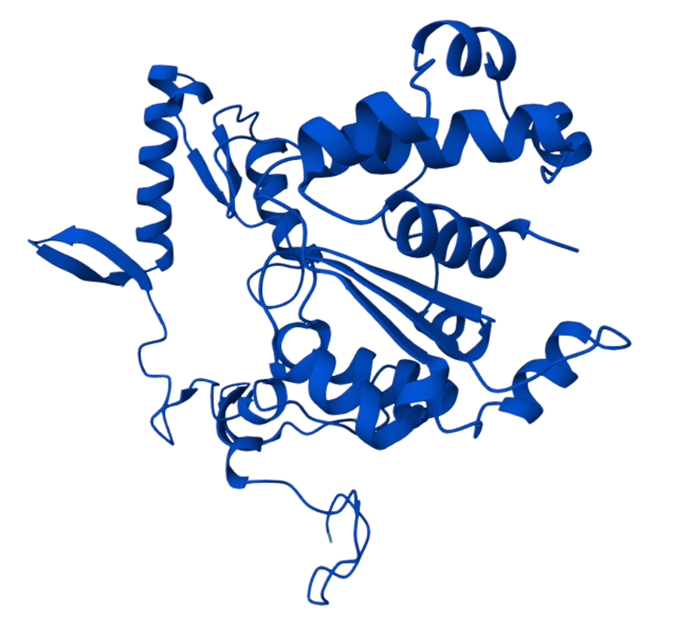
\includegraphics[width=0.5\linewidth]{images/pro0.png}
		\caption{Cấu trúc ba chiều dự đoán của protein được tạo bởi ALPHAFOLD. Mô hình cho thấy cách gấp không gian, cấu trúc xoắn $\alpha$, tấm $\beta$ và tổ chức các miền của protein. Mức độ tin cậy của từng vùng trong cấu trúc được mã hóa màu dựa trên điểm pLDDT, các vùng màu xanh dương thể hiện độ tin cậy cao.}
		\label{fig:pro0}
	\end{figure*}
	
	\section{Kết luận}
	
	Nghiên cứu này đã định danh thành công một chủng vi khuẩn tiềm năng thuộc chi \textit{Ancylobacter} thông qua phân tích trình tự gen 16S rRNA và cây phát sinh loài. Chủng này cho thấy mối quan hệ họ hàng gần gũi với \textit{Ancylobacter novellus}, mở ra khả năng ứng dụng trong các nghiên cứu môi trường liên quan đến arsenic. Trên cơ sở các trình tự ortholog của gen \textit{aioA} thu thập từ các loài vi khuẩn có quan hệ gần gũi, bài nghiên cứu đã xác định được các vùng bảo tồn và thiết kế một cặp mồi PCR đặc hiệu nhằm phát hiện sự hiện diện của gen \textit{aioA} trong chủng vi sinh vật đã phân lập. Đồng thời, phân tích tin sinh học đối với sản phẩm protein được mã hoá đã cung cấp thêm thông tin về đặc điểm sinh hóa và cấu trúc không gian ba chiều tiềm năng của enzyme AioA.
	
	Kết quả nghiên cứu không chỉ cung cấp dữ liệu định danh ban đầu mà còn đặt nền tảng cho việc sàng lọc các chủng vi khuẩn có khả năng oxy hóa arsenite tại Việt Nam. Qua đó, nghiên cứu góp phần định hướng ứng dụng vi sinh vật trong các chiến lược xử lý ô nhiễm arsenite ngoài thực địa theo hướng hiệu quả, chính xác và bền vững trong tương lai.
	
	\section*{Lời cảm ơn}
	Em xin gửi lời cảm ơn sâu sắc tới PGS.TS. Nguyễn Lan Hương và TS. Đàm Thúy Hằng vì đã thiết kế các bài thí nghiệm giàu tính ứng dụng, đồng thời tận tình hướng dẫn em trong quá trình tìm hiểu và sử dụng các công cụ tin sinh học hiện đại trong bài báo cáo này.
	
	\appendices
	Tài liệu bổ sung về các đoạn trình tự gen cũng như các thao tác làm bài được ghi chép trong tệp Word đính kèm.
	
	\printbibliography[title=Tài liệu tham khảo]
	
\end{document}


